\documentclass[a4paper,14pt]{extreport}
	\usepackage[left=1.5cm,right=1.5cm,
	    top=1.5cm,bottom=2cm,bindingoffset=0cm]{geometry}
	\usepackage{scrextend}
	\usepackage[T1,T2A]{fontenc}
	\usepackage[utf8]{inputenc}
	\usepackage[english,russian,ukrainian]{babel}
	\usepackage{tabularx}
	\linespread{1.5}
	\usepackage{amssymb}
	\usepackage{fp}
	\usepackage{color}
	\usepackage{amsmath}
	\usepackage{mathrsfs}
	\usepackage{listings}
	\usepackage{graphicx}
	\graphicspath{ {./images/} }
	\usepackage{lipsum}
	\usepackage{xcolor}
	\usepackage{multirow}
	%\usepackage[table,xcdraw]{xcolor}
	\usepackage{hyperref}
	\usepackage{tcolorbox}
	\usepackage{tikz}
	\usepackage[framemethod=TikZ]{mdframed}
	\usepackage{wrapfig,boxedminipage,lipsum}
	\mdfdefinestyle{MyFrame}{%
	linecolor=blue,outerlinewidth=2pt,roundcorner=20pt,innertopmargin=\baselineskip,innerbottommargin=\baselineskip,innerrightmargin=20pt,innerleftmargin=20pt,backgroundcolor=gray!50!white}
	 \usepackage{csvsimple}
	 \usepackage{supertabular}
	\usepackage{pdflscape}
	\usepackage{fancyvrb}
	%\usepackage{comment}
	\definecolor{ggreen}{rgb}{0.4,1,0}
	\definecolor{rred}{rgb}{1,0.1,0.1}
	\definecolor{aquamarine}{rgb}{0.5, 1.0, 0.83}
	\definecolor{amber}{rgb}{1.0, 0.75, 0.0}
	\definecolor{babyblue}{rgb}{0.54, 0.81, 0.94}
	\definecolor{buff}{rgb}{0.94, 0.86, 0.51}
	\definecolor{internationalorange}{rgb}{1.0, 0.31, 0.0}
	\definecolor{lightmauve}{rgb}{0.86, 0.82, 1.0}
	\definecolor{mediumaquamarine}{rgb}{0.4, 0.8, 0.67}
	\usepackage{array,tabularx}
	\usepackage{colortbl}
	
	\usepackage{varwidth}
	\tcbuselibrary{skins}
	\usepackage{fancybox}

	\usetikzlibrary{calc}
	\makeatletter
	\newlength{\mylength}
	\xdef\CircleFactor{1.1}
	\setlength\mylength{\dimexpr\f@size pt}
	\newsavebox{\mybox}
	\newcommand*\circled[2][draw=blue]{\savebox\mybox{\vbox{\vphantom{WL1/}#1}}\setlength\mylength{\dimexpr\CircleFactor\dimexpr\ht\mybox+\dp\mybox\relax\relax}\tikzset{mystyle/.style={circle,#1,minimum height={\mylength}}}
	\tikz[baseline=(char.base)]
	\node[mystyle] (char) {#2};}
	\makeatother
	\usepackage{pgfplots}
    \pgfplotsset{compat=1.9}


	\usepackage{float}
	\usepackage{wrapfig}
	\usepackage{framed}
	%for nice Code{
	\lstdefinestyle{customc}{
	  belowcaptionskip=1\baselineskip,
	  breaklines=true,
	  frame=L,
	  xleftmargin=\parindent,
	  language=C,
	  showstringspaces=false,
	  basicstyle=\small\ttfamily,
	  keywordstyle=\bfseries\color{green!40!black},
	  commentstyle=\itshape\color{purple!40!black},
	  identifierstyle=\color{blue},
	  stringstyle=\color{orange},
	}
	\lstset{escapechar=@,style=customc}
	\usepackage{enumitem}
%}


\begin{document}
\newtcbox{\xmybox}[1][red]{on line, arc=7pt,colback=#1!10!white,colframe=#1!50!black, before upper={\rule[-3pt]{0pt}{10pt}},boxrule=1pt, boxsep=0pt,left=6pt,right=6pt,top=2pt,bottom=2pt}
\pagecolor{white}
\begin{titlepage}
	\begin{center}
	\large
	Національний технічний університет України \\ "Київський політехнічний інститут імені Ігоря Сікорського"


	Факультет Електроніки

	Кафедра мікроелектроніки
	\vfill

	\textsc{ЗВІТ}\\

	{\Large Про виконання РГР\\
	з дисципліни: «Вакуумна та плазмова електроніка»\\[1cm]

	


	}
	\bigskip
	\end{center}
	\vfill

	\newlength{\ML}
	\settowidth{\ML}{«\underline{\hspace{0.4cm}}» \underline{\hspace{2cm}}}
	\hfill
	\begin{minipage}{1\textwidth}
	Виконавець:\\
	Студент 4-го курсу \hspace{4cm} $\underset{\text{(підпис)}}{\underline{\hspace{0.2\textwidth}}}$  \hspace{1cm}А.\,С.~Мнацаканов\\


	Перевірив: \hspace{5.9cm} $\underset{\text{(підпис)}}{\underline{\hspace{0.2\textwidth}}}$  \hspace{1cm}О.\,М.~Бевза\\

	\end{minipage}

	\vfill

	\begin{center}
	2021
	\end{center}
\end{titlepage}

\begin{center}\textbf{\fbox{Завдання}}\end{center}\par
	\begin{enumerate}
		\item 	Дивимось на графіки побудовані для п.3 лабораторної роботи.
		\begin{enumerate}[label=1.\arabic*]
			\item Визначити частоту червоної границі фотоефекту.
			\item Необхідно визначити напругу запирання для кожного елементу при інтенсивності 50 \% та 100\%.  Пояснити, чому напруги запирання відрізняються при різній інтенсивності.
			\item  Побудувати графіки залежностей напруги запирання від частоти ( у вас вказані довжини хвиль, отже їх треба перерахувати в частоту) для випадку інтенсивності 50\% та 100\%.  Для кожного матеріалу (у кожного свої три матеріала).
			\item Визначити з цих нових побудованих графіків роботу виходу в точці (будь-якій, назвіть її А) за вашим власним вибором, яка розташована десь посередині отриманого графіку. Для всіх трьох матеріалів. Для обох значень інтенсивності (50\% та 100\%). Порівняйте отримані значення роботи виходу при двох різних інтенсивностей для кожного матеріалу та зробити висновки.
			\item  Розрахувати кінетичну швидкість електронів для точки А для всіх трьох матеріалів.
			\item  Порівняти отримане із розрахунку значення роботи виходу з відомими значеннями роботи виходу (довідкові дані, вказати джерело) та розрахувати абсолютну та відносну помилки. Зробити для трьох ваших матеріалів матеріалів.
			\item  Отримані результати звести до таблиці, де повинен бути вказаний кожен з трьох матеріалів та розраховані для нього значення: частота червоної границі фотоефекту, напруга запирання (для двох інтенсивностей), робота виходу в точці А (дві інтенсивності), кінетична швидкість електронів в точці А (для двох інтенсивностей 50\% та 100\%).
			\item Зробіть перевірку правильності виконання розрахунків за формулою Ейнштейна для фотоефекту.
		\end{enumerate}

		\item Беремо  графіки зроблені до пункту 4, де було побудовано залежності струму від інтенсивності. Ви вибирали самі три довжини хвилі. У кожного вибрано свій один матеріал. Робимо:
		\begin{enumerate}[label=2.\arabic*]
			\item Побудуйте ваш графік в інших координатах, де вісь х- довжина хвилі, вісь у-струм. Беремо значення струму для Інтенсивності 50\%.
			\item Побудуйте самі (ваші припущення) на вашому новому графіку іншим кольором як буде виглядати ця залежність, якщо інтенсивність буде складати, а далі за списком вибираємо свій варіант(5-60\%).
		\end{enumerate}
		\item Пояснити чому струм змінився саме так. Дивимось на графіки побудовані для пункта 5. Де залежності енергії від частоти. Треба:
		\begin{enumerate}[label=3.\arabic*]
			\item Визначити яка саме енергія стоїть у вас по осі ігрек. Це повна енергія фотону чи робота виходу чи кінетична енергія електрона чи щось інше? Відповідь аргументовано пояснити.
		\end{enumerate}
\end{enumerate}
\newpage
\begin{center}\textbf{\fbox{Виконання роботи}}\end{center}\par
	
%-----------------------------------------1.1
		\begin{table}[h!]
		\begin{center}
		\caption{Робота виходу даних матеріалів}
			\begin{tabular}{|c|c|}
			\hline
			\textbf{Речовина} & \textbf{Робота виходу, еВ} \\ \hline
			Na                & 2,5                        \\ \hline
			Zn                & 4                          \\ \hline
			Cu                & 4,4                        \\ \hline
			\end{tabular}
			\label{1.2-1.3}
		\end{center}
	\end{table}

	\begin{figure}[h!]
		\center{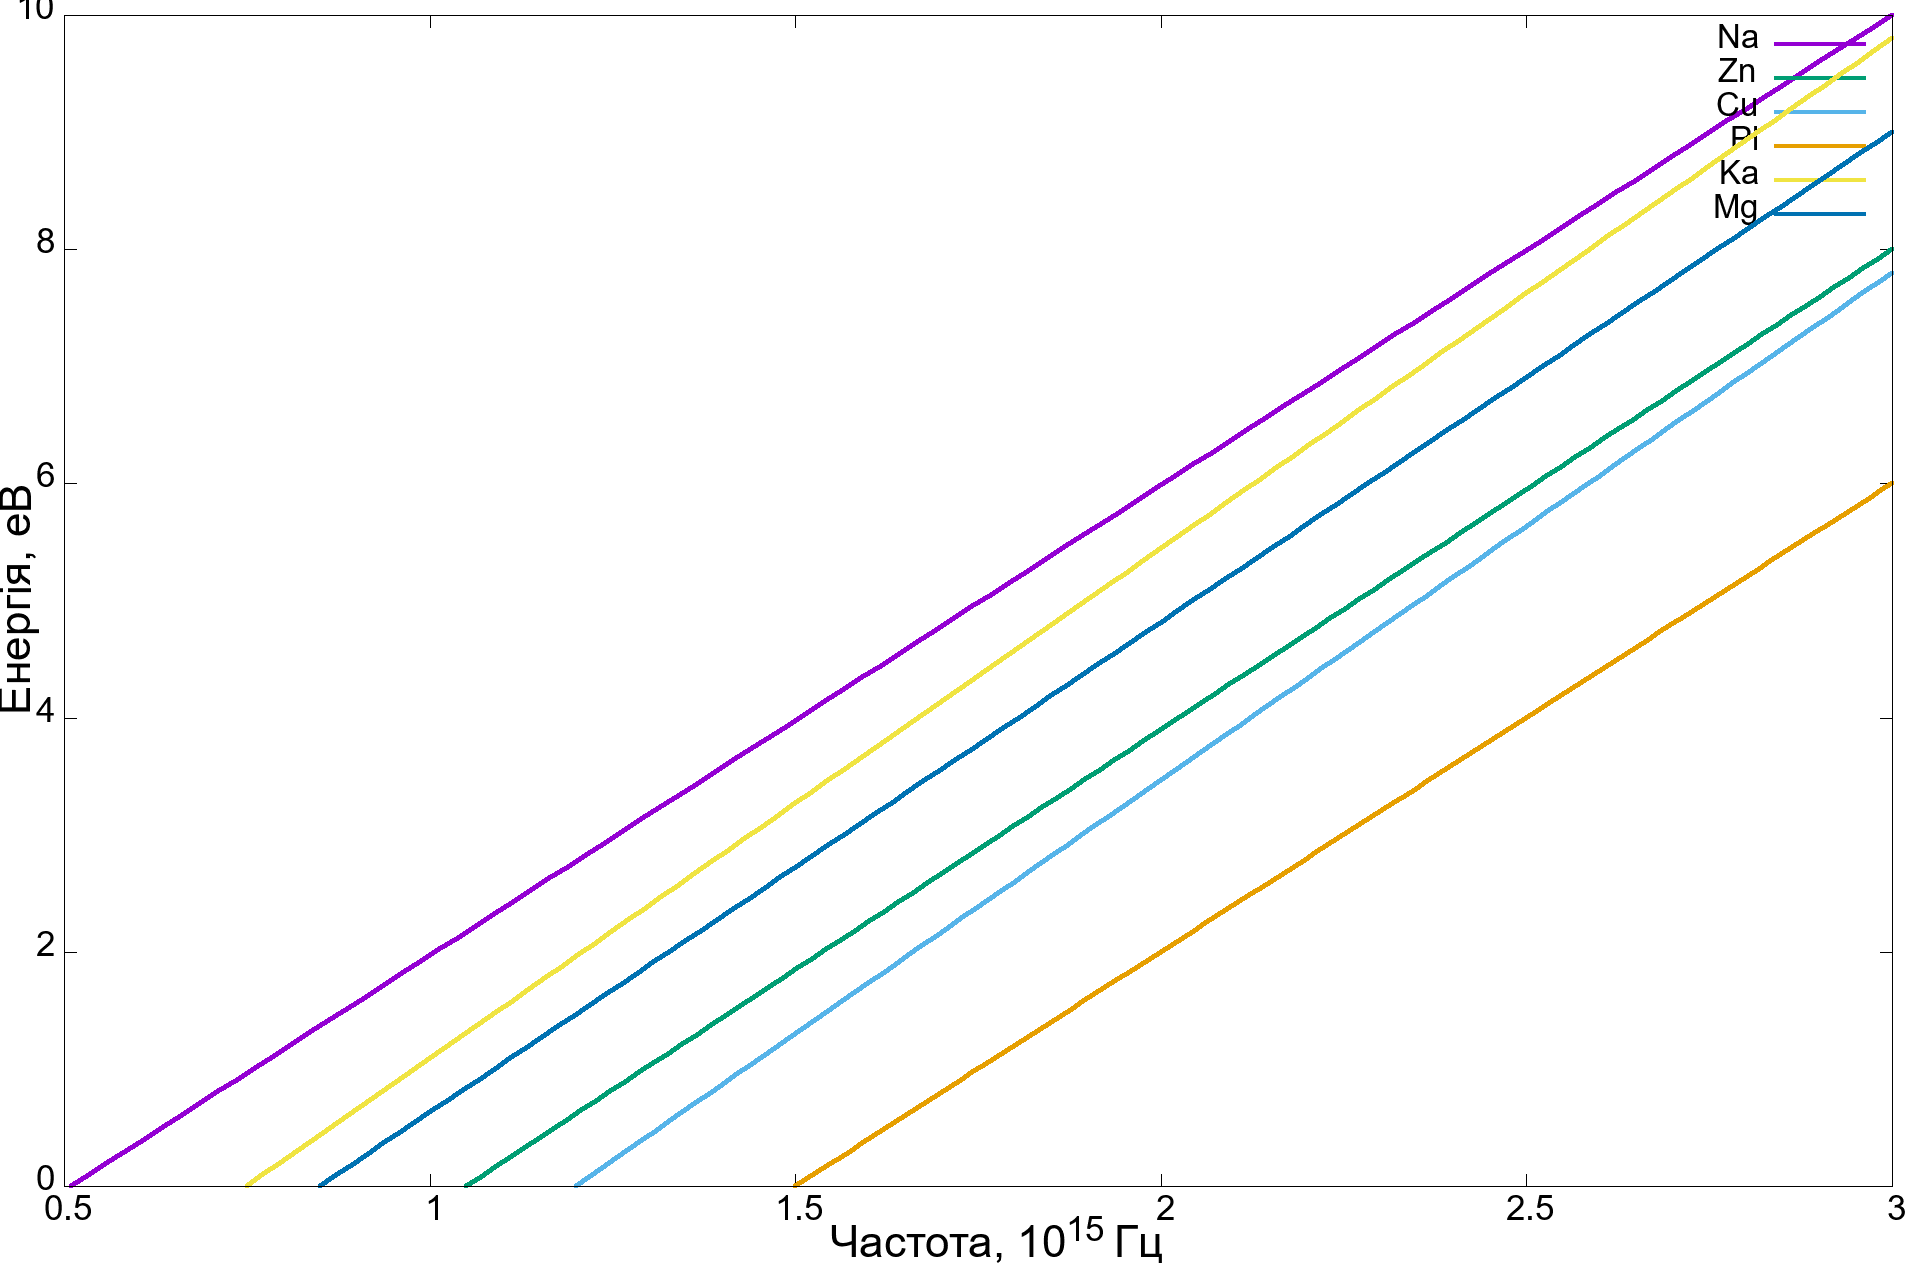
\includegraphics[width=0.5\linewidth]{3part.png}}
		\caption{Ciмейство кривих залежностi Енергiя(частота) при iнтенсивностi 50\% на всьому iнтервалi частот для матерiалiв мiшенi: натрiй, цинк, мiдь, платина, кальцiй, магнiй.}
		\label{ris1}
	\end{figure}
	\begin{center}
		\fcolorbox{black}{aquamarine}{1.1}
	\end{center}
	Використовуючи  рис.\ref{ris1} визначаемо частоту червоної границі фотоефекту.
	\begin{table}[h!]
		\begin{center}
			\caption{Визначення частоти червоної межі фотоефекту}
			\begin{tabular}{|c|c|}
			\hline
			\textbf{Речовина} & \textbf{Частота червоної границі фотоефекту, $10^{15}$ Гц} \\ \hline
			Na                & 0,5                        \\ \hline
			Zn                & 1,1                          \\ \hline
			Cu                & 1,25                        \\ \hline
			\end{tabular}
			\label{tab2}
		\end{center}
	\end{table}

	\clearpage
%-----------------------------------------1.2-1.3
	\begin{center}
		\fcolorbox{black}{aquamarine}{1.2-1.3}
	\end{center}

	За допомогою формули \ref{eq1} знайдемо частоту:
	\begin{equation}{}
		\lambda = \dfrac{c}{v} \text{ } \Rightarrow \text{ } v = \dfrac{c}{\lambda}
		\label{eq1}
	\end{equation}
	\begin{table}[h]
		\begin{center}
			\begin{tabular}{|c|c|}
			\hline
			Довжина хвилі, нм & Частота, $10^{15}$ Гц \\ \hline
			200               & 1,5                   \\ \hline
			400               & 0,75                  \\ \hline
			650               & 0,46                  \\ \hline
			700               & 0,42                  \\ \hline
			\end{tabular}
		\end{center}
	\end{table}
	\begin{table}[h]
			\begin{center}
				\begin{tabular}{|c|c|c|}
					\hline
					\multicolumn{3}{|c|}{\cellcolor[HTML]{DAE8FC}Na} \\ \hline
					 & \multicolumn{2}{c|}{$U_{\text{з}}$, B} \\ \cline{2-3} 
					\multirow{-2}{*}{$f\cdot 10^{15}$, Гц} & 50\% & 100\% \\ \hline
					0.42 & 0 & 0 \\ \hline
					0.46 & 0 & 0 \\ \hline
					0.75 & -5 & -6 \\ \hline
					1.5 & -7.4 & -7.4 \\ \hline
				\end{tabular}
				\begin{tabular}{|c|c|c|}
					\hline
					\multicolumn{3}{|c|}{\cellcolor[HTML]{FFFC9E}Zn} \\ \hline
					\multirow{2}{*}{$f\cdot 10^{15}$, Гц} & \multicolumn{2}{c|}{$U_{\text{з}}$, B} \\ \cline{2-3} 
					 & 50\% & 100\% \\ \hline
					0.42 & 0 & 0 \\ \hline
					0.46 & 0 & 0 \\ \hline
					0.75 & 0 & 0 \\ \hline
					1.5 & -7 & -7 \\ \hline
				\end{tabular}
				\begin{tabular}{|c|c|c|}
					\hline
					\multicolumn{3}{|c|}{\cellcolor[HTML]{9AFF99}Cu} \\ \hline
					\multirow{2}{*}{$f\cdot 10^{15}$, Гц} & \multicolumn{2}{c|}{$U_{\text{з}}$, B} \\ \cline{2-3} 
					 & 50\% & 100\% \\ \hline
					0.42 & 0 & 0 \\ \hline
					0.46 & 0 & 0 \\ \hline
					0.75 & 0 & 0 \\ \hline
					1.5 & -6.2 & -7 \\ \hline
				\end{tabular}
			\end{center}
	\end{table}	

	\begin{minipage}{0.2\textwidth}
		\begin{tikzpicture}%Na
			\begin{axis}[table/col sep = semicolon,
				title={Na},
				xlabel = {$f\cdot 10^{15},\text{ Гц}$},
				ylabel = {$U_{\text{з}}, B$},
				height = 0.25\paperheight, 
				width =  0.25\paperwidth,
				%legend pos = north west,
			    ymajorgrids=true,
			    xmajorgrids=true,
				grid style=dashed,
				legend style={nodes={scale=0.7, transform shape}}]
				\legend{ 
				\text{50\%}, \text{100\%}};
				\addplot table [x={b},y={c}]{1.2-1.3.csv};
				\addplot table [x={b},y={d}]{1.2-1.3.csv};

			\end{axis}
			\draw[thick,black,densely dotted] (1.25,0) -- (1.25,1.42) -- (0,1.42);
			\draw[thick,black,densely dotted] (1.25,0) -- (1.25,2.08) -- 
			(0,2.08);

		\end{tikzpicture}%Na	
	\end{minipage}
	\hfill
	\begin{minipage}{0.2\textwidth}
		\begin{tikzpicture}%Zn
			\begin{axis}[table/col sep = semicolon,
				title={Zn},
				xlabel = {$f\cdot 10^{15},\text{ Гц}$},
				ylabel = {$U_{\text{з}}, B$},
				height =  0.25\paperheight, 
				width =  0.25\paperwidth,
							    ymajorgrids=true,
				    xmajorgrids=true,
	    			grid style=dashed,
	    			legend style={nodes={scale=0.7, transform shape}}]
				\legend{ 
				\text{50\%}, \text{100\%}};
				\addplot table [grid style = both, x={g},y={h}]{1.2-1.3.csv};
				\addplot table [grid style = both, x={g},y={i}]{1.2-1.3.csv};
			\end{axis}
			\draw[thick,black,densely dotted] (2.1,0) -- (2.1,3.3) -- 
			(0,3.3);
			\node [black] at (2.1,3.3) {\textbullet};
		\end{tikzpicture}%Zn
	\end{minipage}
	\hfill
	\begin{minipage}{0.3\textwidth}
		\begin{tikzpicture}%Cu
			\begin{axis}[table/col sep = semicolon,
				title={Cu},
				xlabel = {$f\cdot 10^{15},\text{ Гц}$},
				ylabel = {$U_{\text{з}}, B$},
				height = 0.25\paperheight, 
				width = 0.25\paperwidth,
				ymajorgrids=true,
				xmajorgrids=true,
	    		grid style=dashed,
	    		legend style={nodes={scale=0.7, transform shape}}]
				\legend{ 
				\text{50\%}, \text{100\%}};
				\addplot table [grid style = both, x={l},y={m}]{1.2-1.3.csv};
				\addplot table [grid style = both, x={l},y={n}]{1.2-1.3.csv};
			\end{axis}
			\draw[thick,black,densely dotted] (2.1,0) -- (2.1,3.45) -- 
			(0,3.45);
			\node [black] at (2.1,3.44) {\textbullet};
		\end{tikzpicture}%Cu
	\end{minipage}
%-----------------------------------------1.4
		\begin{center}
			\fcolorbox{black}{aquamarine}{1.4}
		\end{center}	
		Роботу виходу можна знайти за наступною формулою: 
	\begin{equation}
		A = h\cdot f
	\end{equation}

	\FPeval\na{round( 4.14*0.75  :3)}
	\FPeval\naa{round( 4.14*0.7 :3)}

	\FPeval\zn{round( 4.14*1.08  :3)}

	\FPeval\cu{round( 4.14*1.09  :3)}
	\FPeval\cuu{round( 4.14*1.0  :3)}


	\begin{align*}
		A_{Na-50\%} &= \na \text{ eB}\\
		A_{Na-100\%} &= \naa \text{ eB}\\
		A_{Zn} &= \zn \text{ eB}\\
		A_{Cu-50\%} &= \cu \text{ eB}\\
		A_{Cu-100\%} &= \cuu \text{ eB}\\
	\end{align*}
%-----------------------------------------1.5
	\begin{center}
		\fcolorbox{black}{aquamarine}{1.5}
	\end{center}
	Обрахувавши дані за наступною формулою можна отримати кінетичну швидкість електронів для точки А для всіх трьох матеріалів
	\begin{equation}
		\tcbox[nobeforeafter]{$v = \sqrt{ \dfrac{2\cdot e\cdot U_{\text{з}}}{m} }$}
	\end{equation}



	\newtcolorbox{mybox1}[2][]{colback=red!5!white,
	colframe=red!75!black,fonttitle=\bfseries,
	colbacktitle=red!85!black,enhanced,
	attach boxed title to top center={yshift=-2mm},
	title={#2},#1}
	\begin{mybox1}[colback=buff]{Na}
		$$v = \sqrt{ \dfrac{2\cdot 5 \cdot 1.6\cdot 10^{-19} }{9.1\cdot 10^{-31}}} = 13.25\cdot 10^{5} \text{ }\dfrac{\text{м}}{\text{c}} \hspace{1cm}v = 14.52\cdot 10^{5}  \text{ }\dfrac{\text{м}}{\text{c}}$$
	\end{mybox1}

	\begin{mybox1}[colback=mediumaquamarine]{Zn}
		$$v = 10.27\cdot 10^{5}  \text{ }\dfrac{\text{м}}{\text{c}} $$
	\end{mybox1}

	\begin{mybox1}[colback=lightmauve]{Cu}
		$$v =  8.99\cdot 10^{5} \text{ }\dfrac{\text{м}}{\text{c}} \hspace{1cm} v = 9.18\cdot 10^{5}  \text{ }\dfrac{\text{м}}{\text{c}}$$
	\end{mybox1}
%-----------------------------------------1.6
	\newpage
	\begin{center}
		\fcolorbox{black}{aquamarine}{1.6}
	\end{center}

	\begin{table}[h]
	\begin{center}
		\begin{small}
		\begin{tabular}{|c|c|c|c|c|c|}
		\hline
		\multicolumn{2}{|c|}{\cellcolor[HTML]{FFCCC9}Na} & \multicolumn{2}{c|}{\cellcolor[HTML]{FFFFC7}Zn} & \multicolumn{2}{c|}{\cellcolor[HTML]{ECF4FF}Cu} \\ \hline
		\multicolumn{6}{|c|}{A, eB}                                                                                                                          \\ \hline
		розраховане        & з довідника\footnotemark                 & розраховане            & з довідника            & розразоване       & з довідника                 \\ \hline
		3.1                &                             &                        &                        & 4.5               &                             \\ \cline{1-1} \cline{5-5}
		2.8                & \multirow{-2}{*}{2.2}       & \multirow{-2}{*}{4.4}  & \multirow{-2}{*}{4}    & 4.1               & \multirow{-2}{*}{4.4}       \\ \hline
		\multicolumn{6}{|c|}{Похибка}                                                                                                                        \\ \hline
		$\triangle$        & $\delta$                    & $\triangle$            & $\delta$               & $\triangle$       & $\delta$                    \\ \hline
		0.9                & 40\%                        &                        &                        & 0.1               & 2\%                         \\ \cline{1-2} \cline{5-6} 
		0.6                & 27\%                        & \multirow{-2}{*}{0.4}  & \multirow{-2}{*}{10\%} & 0.3               & 6\%                         \\ \hline
		\end{tabular}
		\end{small}
		\end{center}
	\end{table}
	\footnotetext{{Landolt-Borstein's Zahlenwerte und Funktionen aus Phsik, Chemie, Astrunumie, Geophysik, Thechnik, 6-е издание., Берлин, т. I, ч.4, 1955; т. II, ч.6, разд. 1, 1959}}
%-----------------------------------------1.7
		\begin{center}
		\fcolorbox{black}{aquamarine}{1.7}
	\end{center}
	\begin{table}[h]
	\begin{small}
		\begin{tabular}{|l|c|c|c|c|c|c|}
		\hline
		& \multicolumn{2}{c|}{\cellcolor[HTML]{FFCCC9}Na} & \multicolumn{2}{c|}{\cellcolor[HTML]{FFFFC7}Zn} & \multicolumn{2}{c|}{\cellcolor[HTML]{ECF4FF}Cu} \\ \cline{2-7} 
		& \multicolumn{6}{c|}{\cellcolor[HTML]{CBCEFB}A, eB} \\ \cline{2-7} 
		\multirow{-3}{*}{} & розраховане & з довідника & розраховане & з довідника & розразоване & з довідника \\ \hline
		\multicolumn{1}{|c|}{50\%} & 3.1 &  &  &  & 4.5 &  \\ \cline{1-2} \cline{6-6}
		\multicolumn{1}{|c|}{100\%} & 2.8 & \multirow{-2}{*}{2.2} & \multirow{-2}{*}{4.4} & \multirow{-2}{*}{4} & 4.1 & \multirow{-2}{*}{4.4} \\ \hline
		& \multicolumn{6}{c|}{\cellcolor[HTML]{CBCEFB}Частота червоної границі фотоефекту, $10^{15} $ Гц} \\ \cline{2-7} 
		& \multicolumn{2}{c|}{0.5} & \multicolumn{2}{c|}{1.1} & \multicolumn{2}{c|}{1.25} \\ \cline{2-7} 
		\multirow{-3}{*}{} & \multicolumn{6}{c|}{\cellcolor[HTML]{CBCEFB}$U_{\text{з}}$,  В} \\ \hline
		\multicolumn{1}{|c|}{50\%} & \multicolumn{2}{c|}{5} & \multicolumn{2}{c|}{} & \multicolumn{2}{c|}{2.3} \\ \cline{1-3} \cline{6-7} 
		\multicolumn{1}{|c|}{100\%} & \multicolumn{2}{c|}{6} & \multicolumn{2}{c|}{\multirow{-2}{*}{3}} & \multicolumn{2}{c|}{2.4} \\ \hline
		& \multicolumn{6}{c|}{\cellcolor[HTML]{CBCEFB}Кінетична швидкість електронів в точці А, $\cdot 10^{5}  \text{ }\dfrac{\text{м}}{\text{c}}$} \\ \hline
		\multicolumn{1}{|c|}{50\%} & \multicolumn{2}{c|}{13.25} & \multicolumn{2}{c|}{} & \multicolumn{2}{c|}{8.99} \\ \cline{1-3} \cline{6-7} 
		\multicolumn{1}{|c|}{100\%} & \multicolumn{2}{c|}{14.52} & \multicolumn{2}{c|}{\multirow{-2}{*}{10.27}} & \multicolumn{2}{c|}{9.18} \\ \hline
		\end{tabular}	
		\end{small}
	\end{table}
	В даному пункті можна наочно преконатися у другому занконі Столетова, який каже про те, що максимальна кiнетична енергiя
	фотоелектронiв не залежить вiд iнтенсивностi свiтла та лiнiйно зростає з пiдвищенням частоти. Що ми бачимо i в даному випадку: максимальна швидкiсть, що харктеризує максимальну кiнетичну енергiю практично не змiнилась, i лiнiйно зменшується з ростом довжини хвилi.
%-----------------------------------------1.8
	
	
	\begin{center}
		\fcolorbox{black}{aquamarine}{1.8}
	\end{center}
	Зробимо перевiрку правильностi виконання розрахункiв за формулою
	Ейнштейна для фотоефекту:

	\begin{align*}
		hf = A + \dfrac{mv^2}{2}\tetx{  }\Rightarrow \tetx{  } hf -  A =  \dfrac{mv^2}{2}
	\end{align*}

	\begin{align*}
		4.1\cdot 10^{-15}\cdot 1.5\cdot 10^{15} - 3.1 =  \dfrac{9.1\cdot 10^{15}\cdot (13.2\cdot10^5)^2}{2}
	\end{align*}
	
	\begin{align*}
		3.1\text{  eB} \approx  3.8\text{  eB} % 4.2\text{  eB}
	\end{align*}
	Оскільки деякі початкові значення були вибрані не дуже коректно, то присутня невеличка похибка.

%-----------------------------------------2.1 - 2.2

	\begin{center}
		\fcolorbox{black}{aquamarine}{2.1 - 2.2}
	\end{center}

	\begin{center}
		\begin{tikzpicture}%Na
			\begin{axis}[table/col sep = semicolon,
				title={Na},
				xlabel = {Довжина хвилі,\text{ нм}},
				ylabel = {$I_{\text{}}, A$},
				height = 0.3\paperheight, 
				width =  0.3\paperwidth,
				%legend pos = north west,
			    ymajorgrids=true,
			    xmajorgrids=true,
				grid style=dashed,
				legend style={nodes={scale=0.7, transform shape}}]
				\legend{ 
				\text{50\%}, \text{60\%}};
				\addplot table [x={a},y={b}]{2Na_csv.csv};
				\addplot table [x={a},y={c}]{2Na_csv.csv};
			\end{axis}		
		\end{tikzpicture}%Na
	\end{center}
	
	

%-----------------------------------------3
 \newpage
	\begin{center}
		\fcolorbox{black}{aquamarine}{3}
	\end{center}
	
	\begin{figure}[h!]
		\center{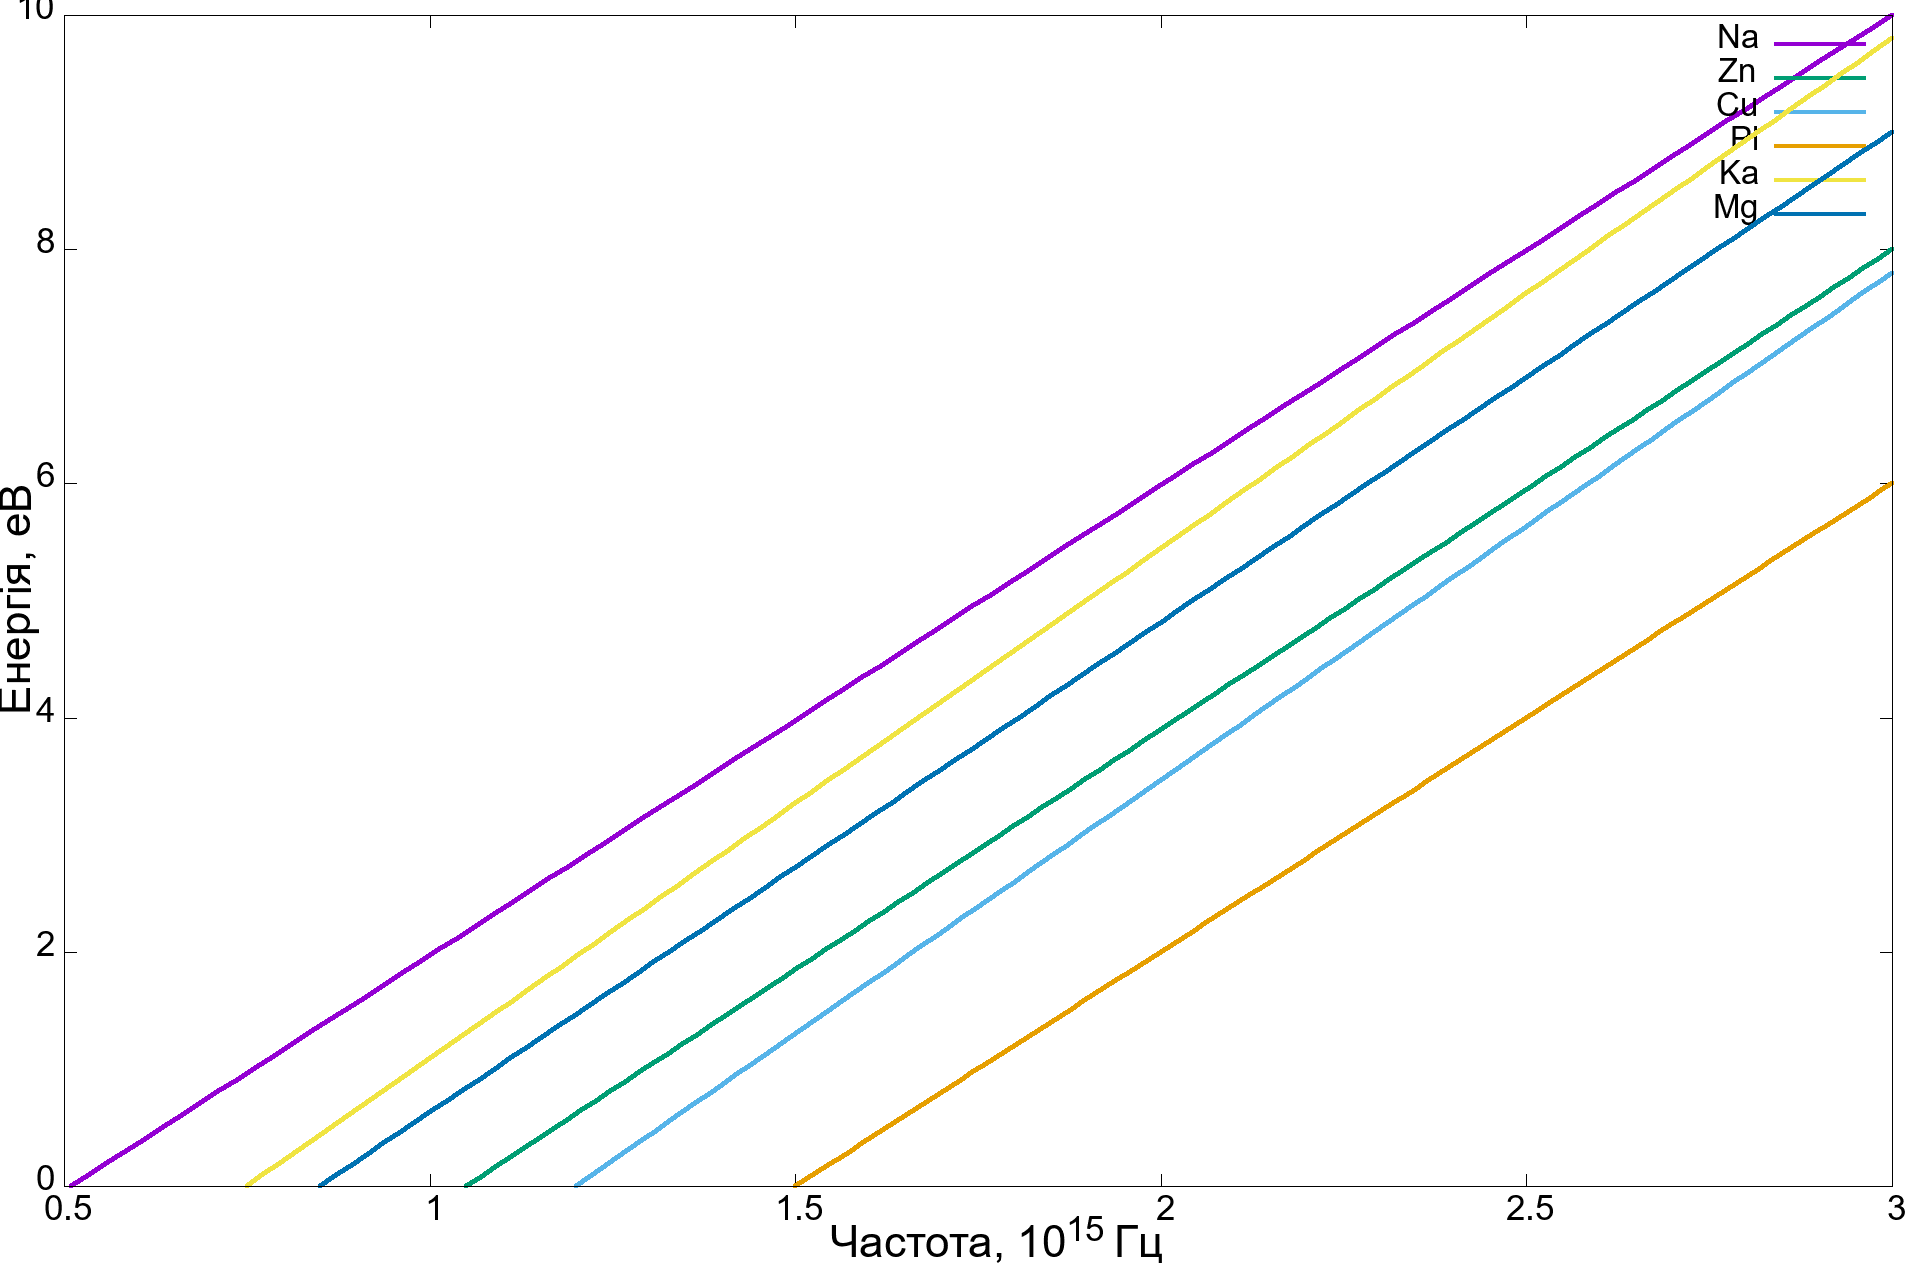
\includegraphics[width=0.6\linewidth]{3part.png}}
		\caption{Ciмейство кривих залежностi Енергiя(частота) }
		\label{ris2}
	\end{figure}

	Виходячи з теоретичних відомостей та засвоєного материалу, можна стверджувати, що по осi Y маэмо максимальну кiнетична енергiю електронiв, це можна легко довести оперуючи II законом Столетова: 
	\emph{ максимальна кiнетична енергiя електрона не залежить
	вiд iнтенсивностi свiтла i лiнiйно збiльшується з ростом частоти}.

%-----------------------------------------1.2
%-----------------------------------------1.2
%-----------------------------------------1.2
%-----------------------------------------1.2














\end{document}
